\subsection{Lower Bounds for Coreset Size in the General Case}

The first result that we will take a look at in the following
theorem shows, that there are some datasets, for which
no sufficiently small coresets of a size of at maximum $k \in O(\log n)$
can be found.

\begin{theorem}
    \label{theorem:index}
    There exists a $d$-dimensional dataset $\mathcal{D}$ of size
    $|\mathcal{D}| = n$, such
    that any $(1+\epsilon)$-coreset $\mathcal{C}$ of $\mathcal{D}$
    for probit regression has a size $k = |\mathcal{C}|$
    of at least $k \in \Omega\left(\frac{n}{\log{n}}\right)$.
\end{theorem}
\begin{proof}
    We can construct such a  dataset by showing
    how coresets can be used in a
    communication protocol for the so called INDEX communication game
    to encode a message.
    The same technique was also used in~\cite{on-coresets} to find
    lower bounds for coresets of logistic regression and is here slightly
    adapted for probit regression.

    The INDEX game consists of two players, Alice and Bob.
    Alice is given a random binary string $m \in \{0, 1\}^n$ of $n$ bits
    and Bob is given an index $i \in [n]$.
    The goal is for Alice to send a message to Bob that allows
    Bob to obtain the value $m_i$ of Alice's binary string $m$.
    It was shown in~\cite{index}, that the minimum length of a message
    sent by Alice that still allows Bob to obtain $m_i$ with
    constant probability is in $\Omega(n)$ bits.
    We will now see, how a coreset for probit regression can be used
    to encode such a message.

    The first step is for Alice to convert her binary string $m$ into
    a two-dimensional dataset $\mathcal{D}$ as follows:
    For each entry $m_j$ of her binary string where $m_j = 1$, she adds
    a point
    \begin{equation*}
        x_j = \left( \cos{\left(2 \pi \frac{j}{n}\right)},
        \sin{\left(2 \pi \frac{j}{n}\right)} \right)^T
    \end{equation*}
    to her set $\mathcal{D}$ and labels it with $y_j = 1$,
    ending up with the dataset
    \begin{equation*}
        \mathcal{D} = \{(x_j, 1)\}_{j \in \{i \in [n]:\ m_i = 1 \}}.
    \end{equation*}
    As we can see, all of these points are on the unit circle and all
    of them are labeled with $1$.

    The next step for her is to construct a
    $(1+\epsilon)$-coreset $\mathcal{C}$ of $\mathcal{D}$
    for probit regression with sample weights $u \in \mathbb{R}^k_{>0}$
    and to transmit both the coreset and the weight vector to Bob,
    which requires $O(\log(n))$ space for each point and
    weight.\footnote{TODO: Why is this a reasonable assumption.}
    We will later see, how
    large the size $|\mathcal{C}|=k$ of this coreset must be,
    so that Bob can still
    obtain the value of $m_i$ with constant probability.

    As soon as Alice's coreset $\mathcal{C}$ arrives at Bob,
    Bob can use it to obtain the value of $m_i$.
    To do this, Bob first adds two new points
    \begin{equation*}
        q_1 = \left( \cos{\left(2 \pi \frac{i - 0.5}{n}\right)},
        \sin{\left(2 \pi \frac{i - 0.5}{n}\right)} \right)^T
    \end{equation*}
    and
    \begin{equation*}
        q_2 = \left( \cos{\left(2 \pi \frac{i + 0.5}{n}\right)},
        \sin{\left(2 \pi \frac{i + 0.5}{n}\right)} \right)^T
    \end{equation*}
    to the set and labels both points with $0$ (see figure~\ref{fig:index}),
    i.e. Bob now has the dataset
    \begin{equation*}
        \mathcal{C}' = \mathcal{C} \cup \{(q_1, 0)\} \cup \{(q_2, 0)\}.
    \end{equation*}

    Next, he uses this new dataset $\mathcal{C}'$ with
    scaled model matrix $C'$ to
    minimize the weighted objective function
    $f_{C'}^u$ of the probit model,
    by using the Newton-Raphson optimization algorithm.

    Taking a look at figure~\ref{fig:index}, it becomes evident,
    that Bobs points $q_1$ and $q_2$ are linearly separable from
    the other points if and only if Alice didn't add a point
    $x_i$, i.e. if $m_i = 0$.
    He can use the results of the optimization procedure to
    make a distinction between the two cases
    (which then allows him to determine the value of $m_i$)
    like this:

    In the case of $m_i=1$, Bobs points are not linearly separable from
    Alices original points, which means that there must occur at least one
    misclassification at a cost of $g(0) = \log(2)$ for the original
    loss function.
    Because Bobs dataset $\mathcal{C}'$ allows him to obtain a
    $(1 \pm \epsilon)$-approximation of the original cost function, he can
    check if the Newton-Raphson algorithm converges to
    a cost of at least $(1 - \epsilon) \log(2) \geq \frac{1}{2} \log(2)$.
    In this case, he knows that Alice must have added the point $x_i$,
    which means that $m_i=1$.

    Conversely, if at any point during the optimization procedure
    the cost function drops below
    $\frac{1}{2} \log(2)$
    and approaches zero, Bob knows that Alice didn't add the point
    $x_i$, because his dataset $\mathcal{C}'$ is linearly separable.
    This will allow him to conclude that $m_i = 0$.

    % There is one special case that has to be dealt with in order for this
    % protocol to work. If Alice's coreset $\mathcal{C}$
    % only consists of the single point
    % $x_i$, Bob's points $q_1$ and $q_2$ could still be linearly seperated
    % although Alice added $x_i$.
    % The workaround to this is simple though:
    % Bob can always just add two more
    % points at the locations of $x_{i-1}$ and $x_{i+1}$ and label them with 1.
    % Now, $q_1$ and $q_2$ can only be linearly seperated from the
    % other points if and only if Alice didn't add a point $x_i$.

    Let us now see how big the size $k$ of Alice's coreset must be
    for this protocol to work with constant probability.
    In~\cite{index} it was shown, that the minimum length of a message
    that Alice must send in order for the protocol to work
    is in $\Omega(n)$ bits.
    Since each of the points that Alice created can be encoded in
    $\log(n)$ space, it follows from the lower bound that
    $\Omega(n) \subseteq \Omega(k \log(n))$, so $k$ must be in
    $\Omega\left(\frac{n}{\log(n)}\right)$.

    We can conclude, that if there existed a $(1 + \epsilon)$-coreset
    of $\mathcal{D}$
    for probit regression with size $k \in o\left(\frac{n}{\log(n)}\right)$,
    it would contradict the minimum message length of
    the INDEX communication game, which proves the theorem.
\end{proof}

\begin{figure}[h]
    \centering
    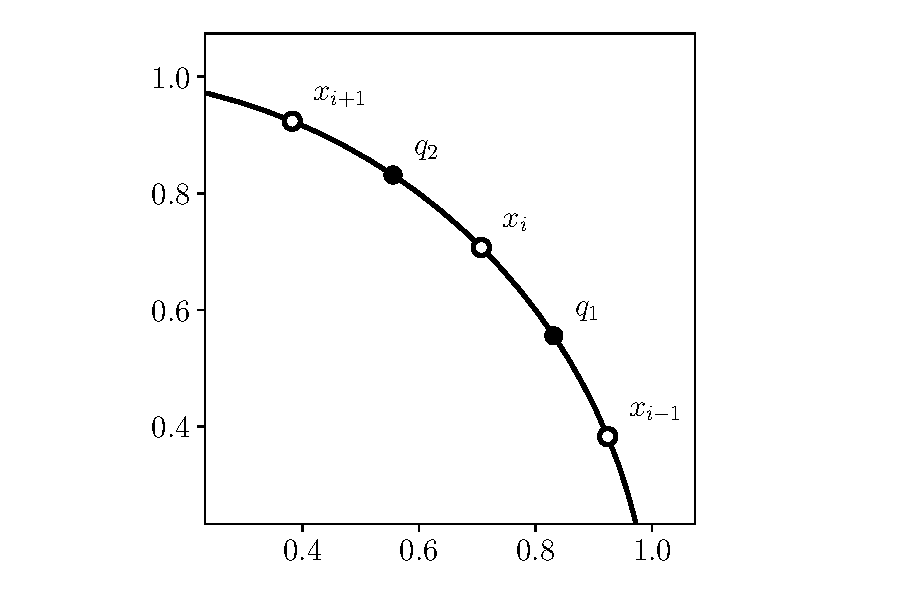
\includegraphics[width=0.8\textwidth]{figures/index.pdf}
    \caption{Bob places two points $q_1$ and $q_2$ in such a way
        on the unit circle, that they can be linearly seperated from the other
        points if and only if Alice didn't place a point at $x_i$.}
    \label{fig:index}
\end{figure}

In the proof of theorem~\ref{theorem:index}, we have already encountered
such a "degenerate" dataset, for which no sublinear sized coreset can be found,
consisting of only positive labels.
The next step of this work is to introduce a new complexity measure
for datasets in the context of probit regression, that allows us
to specify a broad class of datasets for which sublinear sized
coresets do exist and to show how such coresets can be constructed
for this class.
The idea behind this complexity measure goes back to
the work in~\cite{on-coresets}, where the authors introduced a similar
measure to describe a class of datasets that allow the construction
of sublinear coresets in the context of logistic regression.
We adapt this measure to the context of probit regression in the
following definition.

\begin{definition}($\mu$-complexity)
    \label{def:mu}
    Let $\mathcal{D}$ be a $d$-dimensional dataset of size
    $|\mathcal{D}|=n$ with scaled
    model matrix $Z \in \mathbb{R}^{n \times d}$, where
    $z_i \in \mathbb{R}^d$ constitutes the $i$-th
    row of $Z$ and let
    $w \in \mathbb{R}^n_{>0}$ be a vector of positive weights.
    Let $I_\beta^+ = \{i \in [n]:\ w_i z_i^T \beta > 0 \}$
    and let $I_\beta^- = \{i \in [n]:\ w_i z_i^T \beta < 0 \}$.
    Let
    \begin{equation*}
        \mu_w(\mathcal{D}) = \sup_{\beta \in \mathbb{R}^d \setminus \{0\}}
        \frac{\sum_{i \in I_\beta^+} w_i (z_i^T \beta)^2}
        {\sum_{i \in I_\beta^-} w_i (z_i^T \beta)^2}.
    \end{equation*}
    We call the dataset $\mathcal{D}$ with weight vector $w$
    $\mu$-complex, if there exists a $\mu \in \mathbb{R}$,
    such that $\mu_w(\mathcal{D}) \leq \mu$.
\end{definition}

The following lemma will be helpful later on:
\begin{lemma}
    \label{lemma:mu-inequalities}
    Let $\mathcal{D}$ be a $d$-dimensional and $\mu$-complex dataset of size
    $|\mathcal{D}|=n$ with scaled
    model matrix $Z \in \mathbb{R}^{n \times d}$ and weight
    vector $w \in \mathbb{R}^n_{>0}$ like in
    definition~\ref{def:mu}.
    The following relationship holds for all $\beta \in \mathbb{R}^d$:
    \begin{equation*}
        \mu^{-1} \sum_{i \in I_\beta^-} w_i (z_i^T \beta)^2
        \leq \sum_{i \in I_\beta^+} w_i (z_i^T \beta)^2
        \leq \mu \sum_{i \in I_\beta^-} w_i (z_i^T \beta)^2.
    \end{equation*}
\end{lemma}
\begin{proof}
    TODO.
\end{proof}

There is a close relationship between $\mu$ and the linear
separability of a dataset as shown in the following theorem.

\begin{theorem}
    \label{theorem:mu-linear-separability}
    Let $\mathcal{D}$ be a $d$-dimensional dataset of size
    $|\mathcal{D}| = n$ like in definition~\ref{def:mu}
    and let $w \in \mathbb{R}^n_{>0}$ be a vector of
    positive weights.
    Then, the dataset
    $\mathcal{D}$ with weight vector $w$ is $\mu$-complex
    if and only if $\mathcal{D}$ is not linearly separable.
\end{theorem}
\begin{proof}
    We first prove the "$\Rightarrow$" direction, i.e. we show
    that if $\mathcal{D}$ is $\mu$-complex,
    then it is not linearly separable.
    We do this by proving the equivalent
    contraposition that if $\mathcal{D}$ is linearly separable,
    then it is not $\mu$-complex.

    Let $S_0 = \{i \in [n]:\ y_i = 0\}$ and $S_1 = \{i \in [n]:\ y_i = 1\}$
    like in definition~\ref{def:linear-separability}.
    If $\mathcal{D}$ is linearly separable, then there exists
    a $\beta \in \mathbb{R}^d \setminus \{0\}$, such that
    \begin{align*}
                    & \forall i \in S_0:\ x_i^T \beta \leq 0\quad \text{and}\quad \forall i \in S_1:\ x_i^T \beta \geq 0                       \\
        \iff        &                                                                                                                          \\
                    & \forall i \in S_0:\ (-1) x_i^T \beta \geq 0\quad \text{and}\quad \forall i \in S_1:\ x_i^T \beta \geq 0                  \\
        \iff        &                                                                                                                          \\
                    & \forall i \in S_0:\ (2y_i - 1) x_i^T \beta \geq 0\quad \text{and}\quad \forall i \in S_1:\ (2y_i - 1) x_i^T \beta \geq 0 \\
        \iff        &                                                                                                                          \\
                    & \forall i \in S_0:\ z_i^T \beta \geq 0\quad \text{and}\quad \forall i \in S_1:\ z_i^T \beta \geq 0                       \\
        \iff        &                                                                                                                          \\
                    & \forall i \in [n]:\ z_i^T\beta \geq 0                                                                                    \\
        \iff        &                                                                                                                          \\
                    & I_\beta^- = \{ i \in [n]:\ w_iz_i^T\beta < 0\} = \emptyset                                                               \\
        \iff        &                                                                                                                          \\
                    & \sum_{i \in I_\beta^-} w_i (z_i^T \beta)^2 = 0                                                                           \\
        \Rightarrow &                                                                                                                          \\
                    & \mu_w(\mathcal{D}) \geq \frac{\sum_{i \in I_\beta^+} w_i (z_i^T \beta)^2}
        {\sum_{i \in I_\beta^-} w_i (z_i^T \beta)^2} = \infty,
    \end{align*}
    which means that $\mathcal{D}$ is not $\mu$-complex.

    It now remains to prove the "$\Leftarrow$" direction, i.e. to
    show that if $\mathcal{D}$ is not linearly separable,
    then it is $\mu$-complex. Again, we do this by proving the
    equivalent contraposition that if $\mathcal{D}$ is not
    $\mu$-complex, then it is linearly separable.

    The first step in order to do so is to show that we can restrict the
    supremum in $\mu_w(\mathcal{D})$ to finite $\beta$ with
    $\lVert \beta \rVert = 1$:
    \begin{align*}
        \mu_w(\mathcal{D}) & = \sup_{\beta \in \mathbb{R}^d \setminus \{0\}}
        \frac{\sum_{i \in I_\beta^+} w_i (z_i^T \beta)^2}
        {\sum_{i \in I_\beta^-} w_i (z_i^T \beta)^2}                                         \\ & =
        \sup_{\beta \in \mathbb{R}^d \setminus \{0\}}
        \frac{\sum_{i \in I_\beta^+} \frac{1}{\lVert \beta \rVert^2}w_i (z_i^T \beta)^2}
        {\sum_{i \in I_\beta^-} \frac{1}{\lVert \beta \rVert^2} w_i (z_i^T \beta)^2}         \\
                           & =
        \sup_{\beta \in \mathbb{R}^d \setminus \{0\}}
        \frac{\sum_{i \in I_\beta^+} w_i \left(z_i^T \frac{\beta}{\lVert \beta \rVert}\right)^2}
        {\sum_{i \in I_\beta^-}  w_i \left(z_i^T \frac{\beta}{\lVert \beta \rVert}\right)^2} \\
                           & =
        \sup_{\tilde\beta \in \mathbb{R}^d,\ \lVert \tilde\beta \rVert = 1}
        \frac{\sum_{i \in I_\beta^+} w_i \left(z_i^T \tilde\beta \right)^2}
        {\sum_{i \in I_\beta^-}  w_i \left(z_i^T \tilde\beta \right)^2},
    \end{align*}
    which lets us conclude that even in the supremum, both expressions
    $\sum_{i \in I_\beta^+} w_i (z_i^T \beta )^2$
    and
    $\sum_{i \in I_\beta^-}  w_i (z_i^T \beta )^2$
    are finite.
    This means that if $\mathcal{D}$ is not $\mu$-complex, then
    the denominator must be zero, i.e. it must hold that there exists
    a $\beta \in \mathbb{R}^d \setminus \{0\}$ such that
    \begin{equation*}
        \sum_{i \in I_\beta^-}  w_i (z_i^T \beta )^2 = 0.
    \end{equation*}

    From here, we can follow the same chain of equivalences that we
    showed when proving the "$\Rightarrow$"-direction of the theorem,
    which leads us directly to the fact, that $\mathcal{D}$ in this case must
    be linearly separable, which concludes the proof.
\end{proof}

As we already noted in section~\ref{sec:parameter-estimation},
linear separability is also closely related to the existence
of the maximum likelihood estimate in the probit model.
The next theorem uses the relationship between $\mu$ and
linear separability to show the connection between $\mu$
and the existence of the maximum likelihood estimate.

\begin{theorem}
    Let $\mathcal{D}$ be a $d$-dimensional dataset.
    Then, the maximum likelihood estimate $\tilde\beta$ for the probit
    model exists if and only if $\mathcal{D}$ is $\mu$-complex.
\end{theorem}
\begin{proof}
    This is a direct corollary from theorem~\ref{theorem:probit-existence}
    and theorem~\ref{theorem:mu-linear-separability}.
\end{proof}

In the following parts of this work, we will derive efficient upper
bounds on the coreset size for $\mu$-complex datasets.
In order to do this, we first introduce a theoretic
framework that we use for the coreset construction which
is based on the concept of sensitivities.